% Chapter 12. The five jobs of a host, and where each one sits.
\documentclass[tikz,border=6pt]{standalone}
% Shared look for every TikZ figure in the book.
% Colours match book/preamble.tex exactly. Change both or neither.

\usepackage{tikz}
\usepackage{xcolor}
\usepackage{amsmath}
\IfFileExists{libertinus.sty}{\usepackage[mono=false]{libertinus}}{}
\IfFileExists{inconsolata.sty}{\usepackage[varqu,varl,scaled=0.95]{inconsolata}}{}

\usetikzlibrary{
  arrows.meta, positioning, calc, fit, backgrounds, shapes.geometric,
  shapes.misc, decorations.pathreplacing, decorations.pathmorphing,
  patterns, chains, matrix, shadows.blur
}

\definecolor{ink}{HTML}{15181D}
\definecolor{muted}{HTML}{5B6472}
\definecolor{rule}{HTML}{C9CED6}
\definecolor{wash}{HTML}{F4F5F7}
\definecolor{accent}{HTML}{0F5C8C}
\definecolor{accentsoft}{HTML}{E7F0F6}
\definecolor{warm}{HTML}{B4531A}
\definecolor{warmsoft}{HTML}{FBF0E7}
\definecolor{good}{HTML}{2C6E49}
\definecolor{goodsoft}{HTML}{E9F2EC}
\definecolor{danger}{HTML}{9B2226}
\definecolor{dangersoft}{HTML}{FAECEC}

\tikzset{
  font=\sffamily\small,
  >={Stealth[length=5pt, width=4pt]},
  %
  box/.style={
    draw=rule, line width=0.8pt, fill=wash, rounded corners=2pt,
    inner sep=7pt, align=center, text=ink, minimum height=9mm,
  },
  boxa/.style={box, draw=accent, fill=accentsoft},
  boxg/.style={box, draw=good,   fill=goodsoft},
  boxw/.style={box, draw=warm,   fill=warmsoft},
  boxd/.style={box, draw=danger, fill=dangersoft},
  %
  lane/.style={draw=rule, line width=0.7pt, fill=white, rounded corners=2pt,
               inner sep=6pt, align=center, minimum width=26mm},
  %
  flow/.style={draw=accent, line width=1.0pt, ->},
  flowback/.style={flow, densely dashed},
  flowmuted/.style={draw=muted, line width=0.8pt, ->},
  lifeline/.style={draw=rule, line width=0.7pt, densely dotted},
  %
  lbl/.style={font=\sffamily\scriptsize, text=muted, inner sep=2pt},
  lblink/.style={font=\sffamily\scriptsize, text=ink, inner sep=2pt},
  tag/.style={font=\ttfamily\scriptsize, text=accent, inner sep=2pt,
              fill=white, inner xsep=3pt},
  note/.style={font=\sffamily\scriptsize\itshape, text=muted, align=left},
  %
  band/.style={draw=none, rounded corners=1pt},
  tick/.style={draw=muted, line width=0.6pt},
}

% A horizontal timeline bar segment: \barseg{x0}{x1}{y}{colour}{label}
\newcommand{\barseg}[5]{%
  \fill[#4, rounded corners=1pt] (#1,#3-0.16) rectangle (#2,#3+0.16);
  \node[lbl, text=white, font=\sffamily\scriptsize\bfseries]
       at ({(#1+#2)/2},#3) {#5};
}

\begin{document}
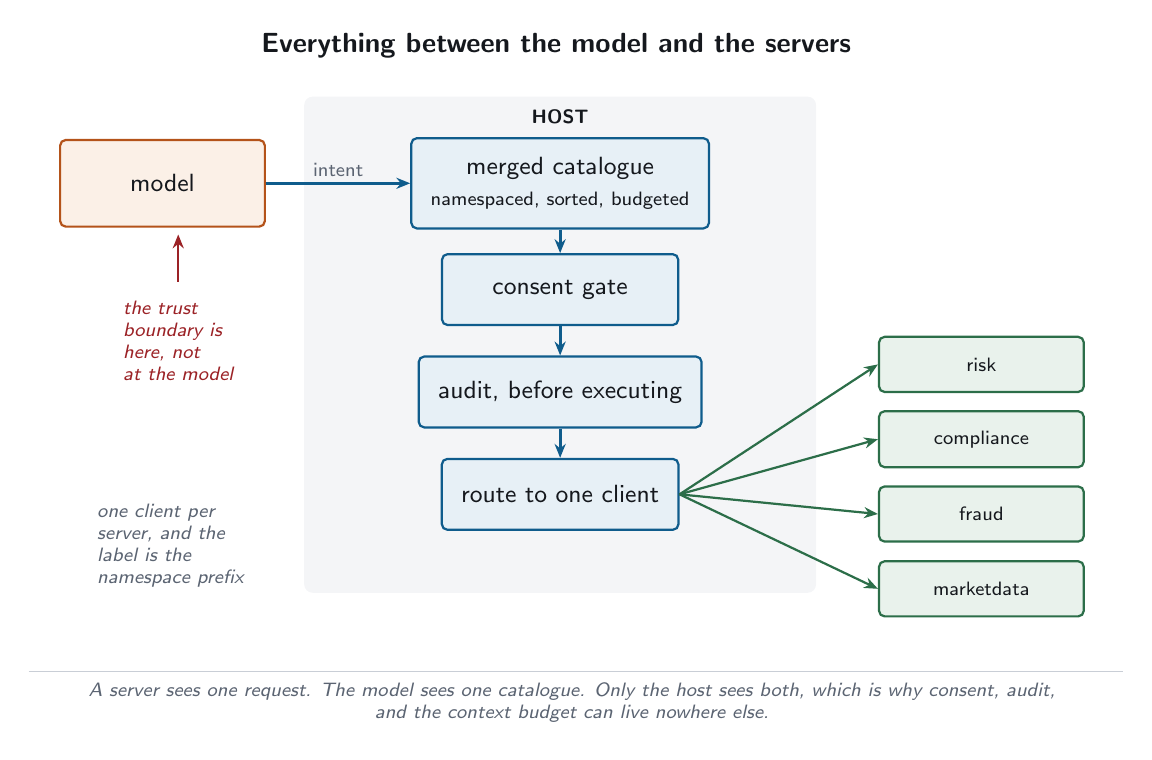
\begin{tikzpicture}[x=1cm, y=1cm]

  \node[lblink, font=\sffamily\bfseries] at (5.2,5.35) {Everything between the model and the servers};

  \node[boxw, minimum width=26mm, minimum height=11mm] (model) at (0.2,3.6) {model};

  \begin{scope}[on background layer]
    \fill[wash, rounded corners=3pt] (2.0,-1.6) rectangle (8.5,4.7);
  \end{scope}
  \node[lbl, font=\sffamily\scriptsize\bfseries, text=ink] at (5.25,4.45) {HOST};

  \node[boxa, minimum width=30mm] (cat)     at (5.25,3.6)  {merged catalogue\\{\scriptsize namespaced, sorted, budgeted}};
  \node[boxa, minimum width=30mm] (consent) at (5.25,2.25) {consent gate};
  \node[boxa, minimum width=30mm] (audit)   at (5.25,0.95) {audit, before executing};
  \node[boxa, minimum width=30mm] (route)   at (5.25,-0.35) {route to one client};

  \draw[flow] (model.east) -- node[lbl, above, pos=0.5] {intent} (cat.west);
  \draw[flow] (cat) -- (consent);
  \draw[flow] (consent) -- (audit);
  \draw[flow] (audit) -- (route);

  \foreach \i/\y/\n in {0/1.3/risk, 1/0.35/compliance, 2/-0.6/fraud, 3/-1.55/marketdata} {
    \node[boxg, minimum width=26mm, minimum height=7mm, font=\sffamily\scriptsize]
      (s\i) at (10.6,\y) {\n};
    \draw[flowmuted, draw=good] (route.east) -- (s\i.west);
  }

  \node[note, align=left, text=danger] at (0.4,1.6)
    {the trust\\boundary is\\here, not\\at the model};
  \draw[flowmuted, draw=danger] (0.4,2.35) -- (0.4,2.95);

  \node[note, align=left] at (0.3,-1.0)
    {one client per\\server, and the\\label is the\\namespace prefix};

  \draw[rule, line width=0.7pt] (-1.5,-2.6) -- (12.4,-2.6);
  \node[note, align=center, text=muted] at (5.4,-3.0)
    {A server sees one request. The model sees one catalogue. Only the host
     sees both, which is why consent, audit,\\and the context budget can live
     nowhere else.};

\end{tikzpicture}
\end{document}
